\section{Results}
%\subsection{Elastic Scattering}

A benchmark region of interest is defined between the upper and lower thresholds in cS1 for each channel. This region
is bounded in $y$-space from above by the $^{241}$AmBe NR mean line and below by the lower 3$\sigma$ quantile of the $^{241}$AmBe neutron calibration data. The expected background in the region is $3 \pm 0.5$ (low-energy) and $1.41 \pm 0.28$ (high-energy). The number of DM candidates in this benchmark region is 3 (low-energy), and 0 (high-energy). The data is compatible with the background-only hypothesis and no excess is found. 

For the elastic scattering case, a 90\%\,CL$_S$~\cite{cls} confidence limit is set on the effective coupling constant, $c_i$,  for all operators and masses in the range of 10~GeV/$c^2$ to 1 TeV/$c^2$. 
%\Xehund\ sets the strongest limits. % tomorrow another experiment will be better.
These limits are shown in Fig.~\ref{fig:elasticLimit} in black, along with limits from CDMS-II Si, CDMS-II Ge and SuperCDMS~\cite{CDMSEFT}.  

\RanComment{A higher energy range of up to 1000~PE is examined as well. There are no NR candidates in that region as well. Notice that we do not use the region above 180~PE as the NR calibration sample is too small, however once higher NR calibration data is available more stringent limits can be produced.}
\begin{figure}
%\centerline{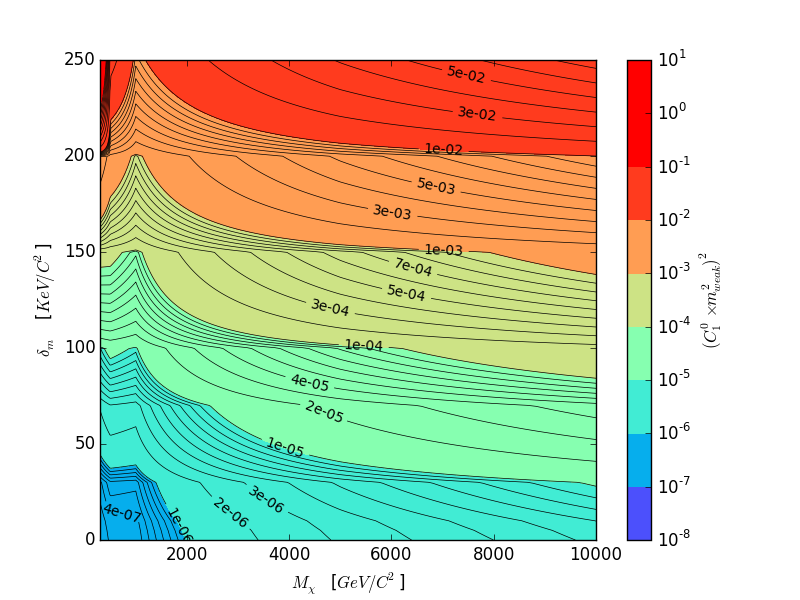
\includegraphics[width=1.\linewidth]{Figures/inelastic_delta_vs_m.png}}
\centerline{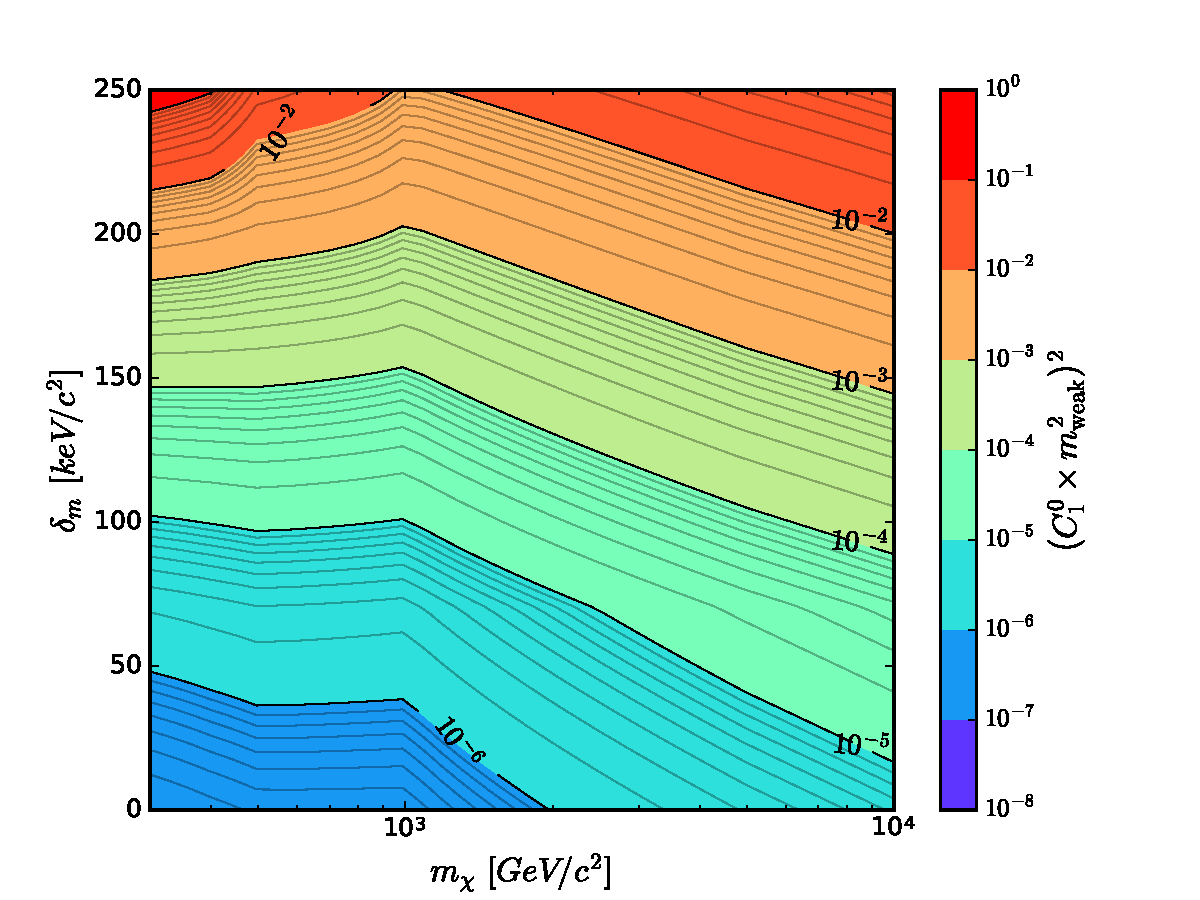
\includegraphics[width=1.\linewidth]{Figures/O1_inelastic_lim_2D}}
\caption{90\%\,CL$_S$ limits, for the inelastic model, on the magnitude of the coupling constant for $\mathcal{O}_1$, reported as a function of the WIMP mass and mass splitting $\delta$.}
\label{fig:O1Inel}
\end{figure}  

For the inelastic scattering case, 90\%\,CL$_S$ confidence limits on the coupling constants are set. Fig.~\ref{fig:O1Inel} shows limits on the $\mathcal{O}_1$ (SI) coupling constant as a function of mass splitting and WIMP mass, Fig.~\ref{fig:InelasticLimit} shows limits for all other operators as a function of the mass splitting $\delta_m$ with a fixed WIMP mass of 1 TeV/$c^2$.  

\begin{figure*}
\begin{minipage}{1.\linewidth}{}
\centerline{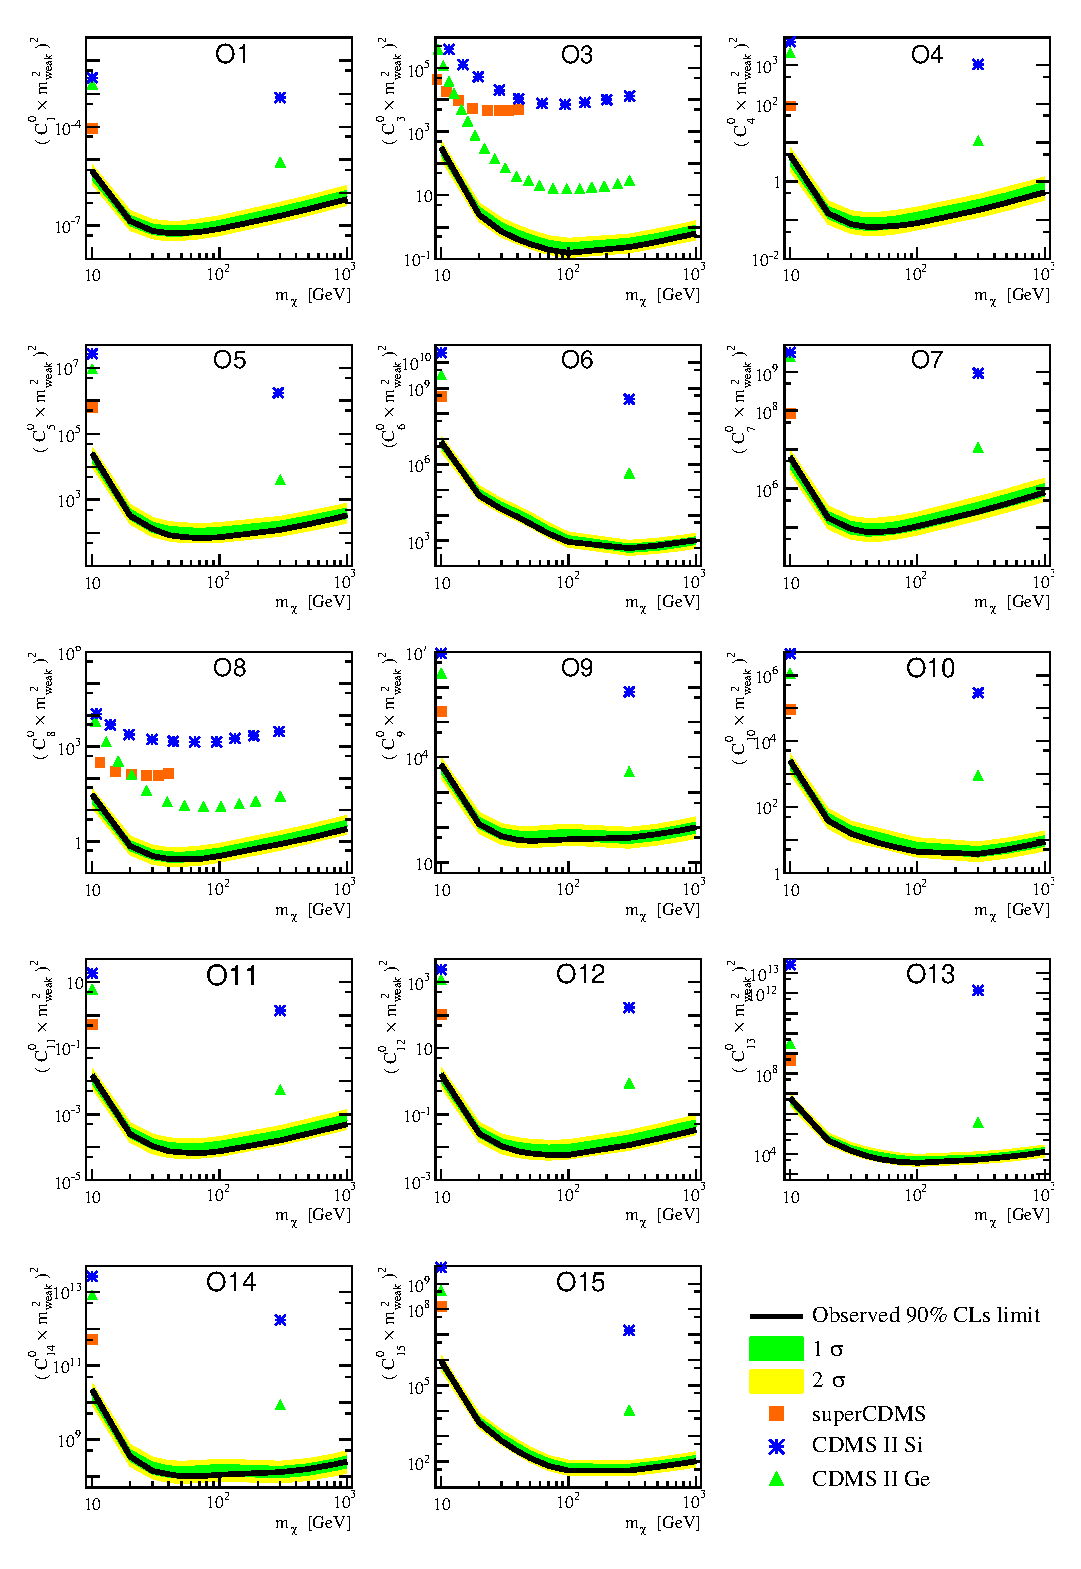
\includegraphics[width=\textwidth,height=0.99\textheight,keepaspectratio]{Figures/ElasticAllLimitCDMS.eps}}
\end{minipage}
\caption{The \Xehund\ limits (90\%\,CL$_S$) on isoscalar dimensionless coupling for all elastic scattering EFT operators. The limits are indicated in solid black. The expected sensitivity is shown in green and yellow(1$\sigma$ and 2$\sigma$ respectively). Limits from CDMS-II Si, CDMS-II Ge, and SuperCDMS \cite{CDMSEFT} are presented as blue asterisks, green triangles, and orange rectangles, respectively (color online). For operator 3 and 8 a full limit from CDMS is published and indicated by a dashed line in the respective colors.}
\label{fig:elasticLimit}
\end{figure*}

\begin{figure*}
\begin{minipage}{1.\linewidth}
\centerline{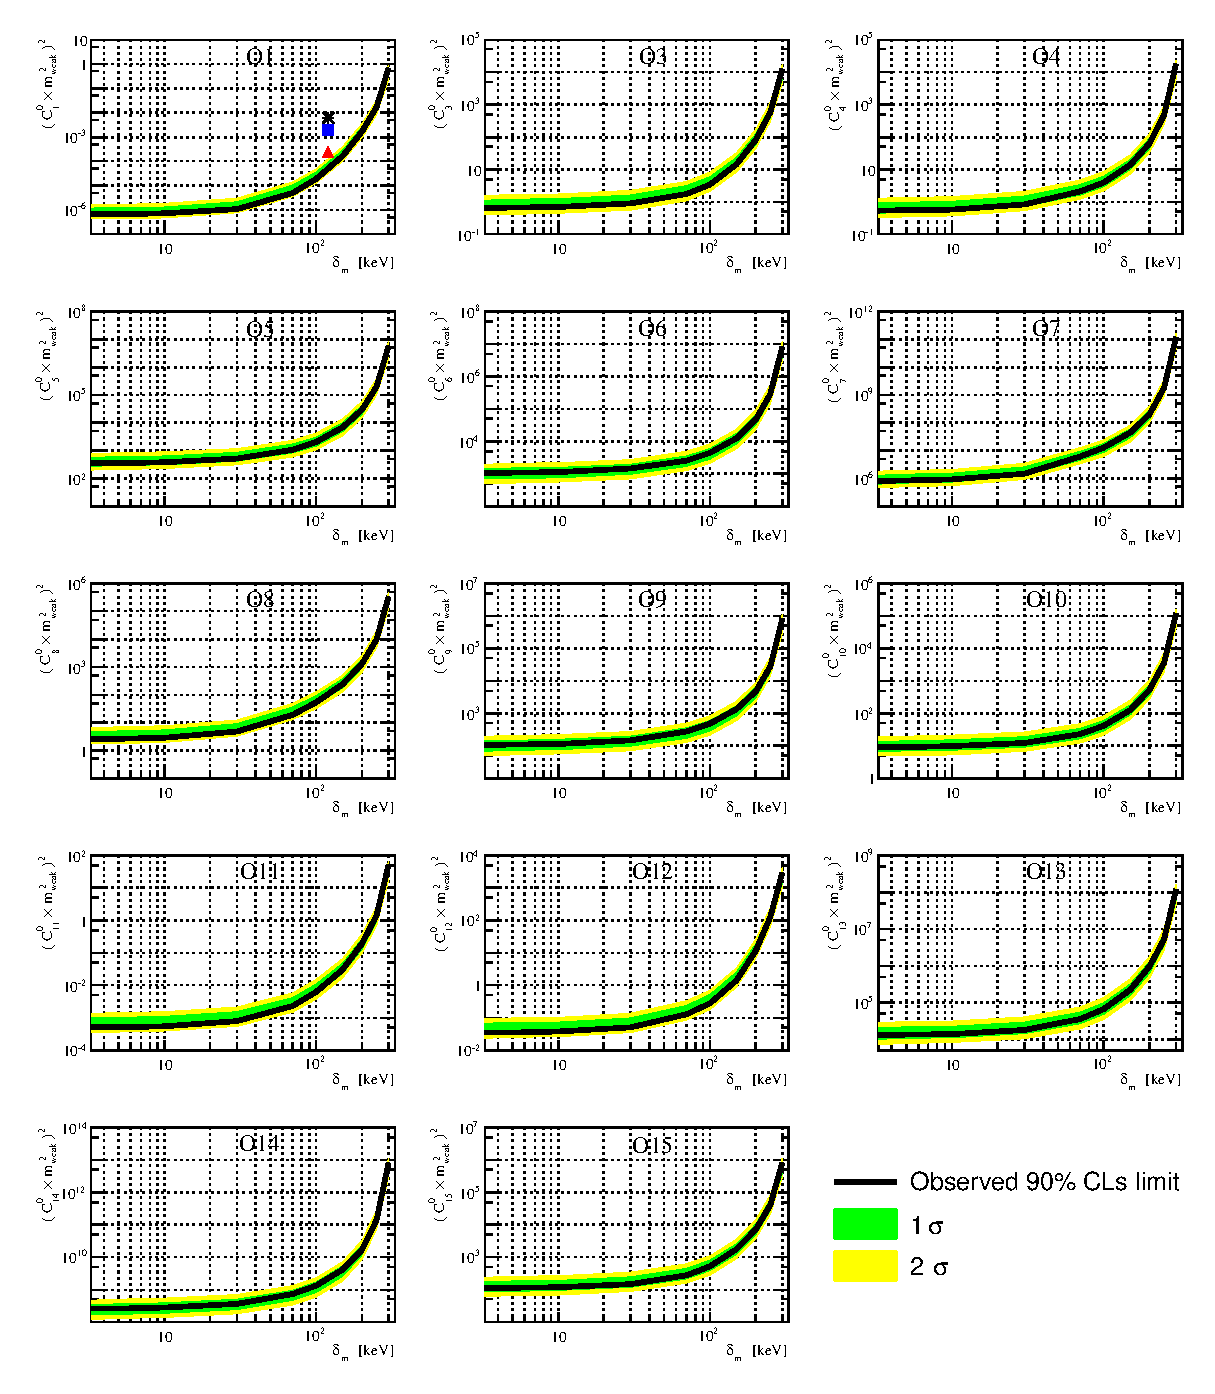
\includegraphics[width=\textwidth,height=0.99\textheight,keepaspectratio]{Figures/FinalInelastic.eps}}
\end{minipage}
\caption{The \Xehund\ 90\%\,CL$_S$ limits on a 1 TeV/$c^2$ WIMP isoscalar dimensionless coupling as function of the WIMP mass splitting $\delta_m$  for all inelastic scattering EFT operators. Limits are indicated in solid black. The expected sensitivity is shown in green and yellow (1$\sigma$ and 2$\sigma$ respectively).}
\label{fig:InelasticLimit}
\end{figure*}


% \begin{figure*}
% \begin{minipage}{1.\linewidth}
% \centerline{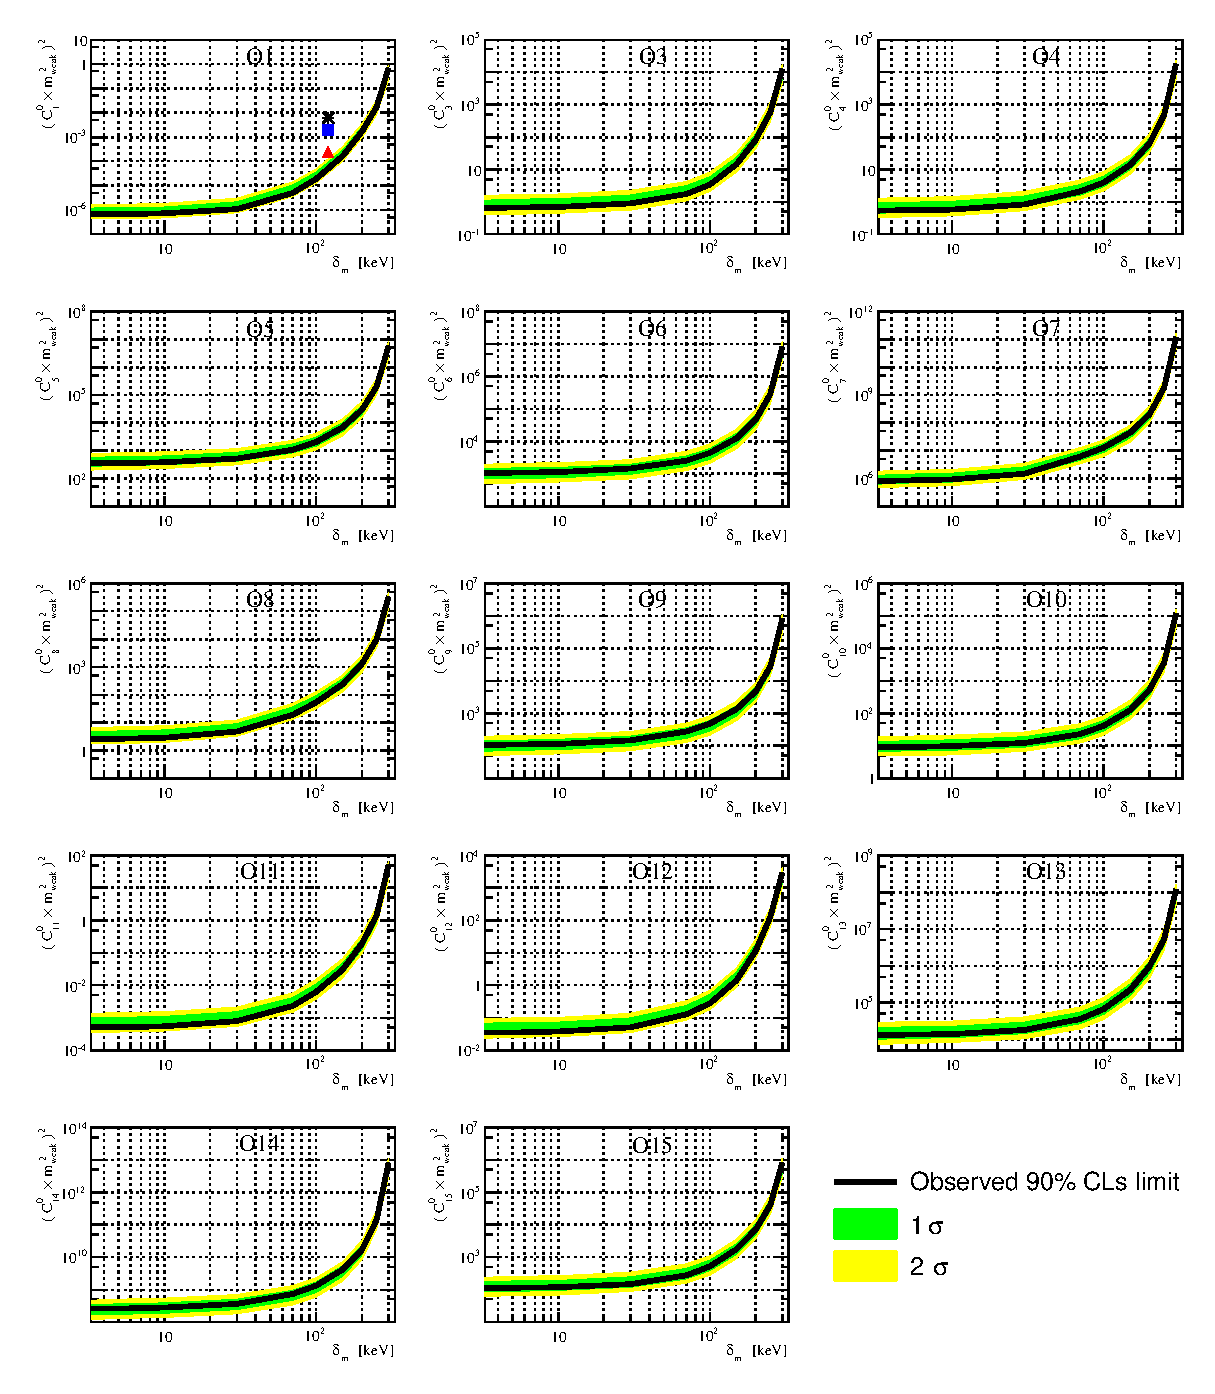
\includegraphics[width=\textwidth,height=0.95\textheight,keepaspectratio]{Figures/FinalInelastic.eps}}
% \end{minipage}
% \caption{The \Xehund\ 90\%\,CL$_S$ limits on a 1 TeV/$c^2$ WIMP isoscalar dimensionless coupling for all inelastic scattering EFT operators. Limits are indicated in solid black. The expected sensitivity is shown in green and yellow (1$\sigma$ and 2$\sigma$ respectively).}
% \label{fig:InelasticLimit}
% \end{figure*}

%\FloatBarrier

